\chapter{概率与统计基础}

\intro{概率论与统计学为深度学习提供了描述不确定性的数学语言。许多损失函数（如交叉熵）可以从概率角度推导出来，生成模型直接建模数据的概率分布，而贝叶斯方法则为模型选择提供了统一框架。本章介绍随机变量、常见分布、条件概率与贝叶斯定理、期望与方差、信息论基础，以及最大似然估计等内容。}

\section{随机变量与概率分布}

\subsection{离散随机变量}

\begin{mydefinition}{离散随机变量与概率质量函数}
离散随机变量 $X$ 取有限或可数无限个值。其概率质量函数（PMF）定义为：
\[
P(X=x)=p_X(x), \quad \sum_{x} p_X(x) = 1
\]
其中 $p_X(x)\in[0,1]$ 对于所有 $x$。
\end{mydefinition}

常见的离散分布：

\begin{itemize}
    \item \textbf{Bernoulli 分布}：描述单次二值试验。$X\in\{0,1\}$，$P(X=1)=p$，$P(X=0)=1-p$。PMF：$p_X(x)=p^x(1-p)^{1-x}$。
    \item \textbf{二项分布}：$n$ 次独立 Bernoulli 试验中成功的次数。$X\sim\text{Binomial}(n,p)$，$P(X=k)=\binom{n}{k}p^k(1-p)^{n-k}$。
    \item \textbf{多项分布}：二项分布向多类别的推广。每个类别 $k$ 有概率 $p_k$，$\sum_k p_k=1$。
    \item \textbf{Poisson 分布}：描述单位时间内随机事件发生的次数。$P(X=k)=\frac{\lambda^k e^{-\lambda}}{k!}$，$\lambda>0$。
    \item \textbf{类别分布（Categorical）}：深度学习中分类问题的输出分布。$P(X=k)=p_k$，$\sum_{k=1}^{K}p_k=1$。当 $K=2$ 时退化为 Bernoulli 分布。
\end{itemize}

\subsection{连续随机变量}

\begin{mydefinition}{连续随机变量与概率密度函数}
连续随机变量 $X$ 的概率密度函数（PDF）$f_X(x)$ 满足 $f_X(x)\geq 0$ 且：
\[
\int_{-\infty}^{\infty} f_X(x)\,dx = 1
\]
$X$ 落在区间 $[a,b]$ 内的概率为 $P(a\leq X\leq b)=\int_a^b f_X(x)\,dx$。
\end{mydefinition}

常见的连续分布：

\begin{itemize}
    \item \textbf{均匀分布}：$X\sim U(a,b)$，PDF：$f_X(x)=\frac{1}{b-a}$，$x\in[a,b]$。
    \item \textbf{正态分布（高斯分布）}：$X\sim\mathcal{N}(\mu,\sigma^2)$，PDF：
    \[
    f_X(x)=\frac{1}{\sqrt{2\pi\sigma^2}}\exp\left(-\frac{(x-\mu)^2}{2\sigma^2}\right)
    \]
    \item \textbf{多元正态分布}：$\mathbf{X}\sim\mathcal{N}(\boldsymbol{\mu},\boldsymbol{\Sigma})$，PDF：
    \[
    f_{\mathbf{X}}(\mathbf{x})=\frac{1}{(2\pi)^{n/2}|\boldsymbol{\Sigma}|^{1/2}}\exp\left(-\frac{1}{2}(\mathbf{x}-\boldsymbol{\mu})^{\top}\boldsymbol{\Sigma}^{-1}(\mathbf{x}-\boldsymbol{\mu})\right)
    \]
    \item \textbf{指数分布}：描述等待时间。$f_X(x)=\lambda e^{-\lambda x}$，$x\geq 0$。
    \item \textbf{Laplace 分布}：$f_X(x)=\frac{1}{2b}\exp(-\frac{|x-\mu|}{b})$，常用于 $L^1$ 正则化的贝叶斯解释。
\end{itemize}

\begin{figure}[H]
\centering
\begin{tikzpicture}[
    mycurve/.style={thick, smooth},
    mylabel/.style={font=\small}
]
    % Axes
    \draw[->, >=stealth] (-5, 0) -- (5, 0) node[right] {$x$};
    \draw[->, >=stealth] (0, 0) -- (0, 4.5) node[above] {$f_X(x)$};

    % Gaussian mu=0, sigma=1
    \draw[mycurve, blue!70, domain=-4.5:4.5, samples=100]
        plot (\x, {4*exp(-\x*\x/2)/sqrt(2*pi)});

    % Gaussian mu=0, sigma=0.5 (narrower)
    \draw[mycurve, red!70, domain=-4:4, samples=100]
        plot (\x, {4*exp(-\x*\x/0.5)/sqrt(0.5*pi)});

    % Gaussian mu=1.5, sigma=1
    \draw[mycurve, green!50!black, domain=-3.5:6, samples=100]
        plot (\x, {4*exp(-(\x-1.5)*(\x-1.5)/2)/sqrt(2*pi)});

    % Labels
    \node[mylabel, blue!70] at (2.5, 1.8) {$\mathcal{N}(0,1)$};
    \node[mylabel, red!70] at (1.5, 3.2) {$\mathcal{N}(0,0.25)$};
    \node[mylabel, green!50!black] at (5.5, 1.5) {$\mathcal{N}(1.5,1)$};

    % Standard deviations
    \draw[blue!70, dashed] (-1, 0) -- (-1, {4*exp(-0.5)/sqrt(2*pi)});
    \draw[blue!70, dashed] (1, 0) -- (1, {4*exp(-0.5)/sqrt(2*pi)});
    \node[mylabel, blue!70] at (0, -0.5) {$68\%$};

    \node[mylabel] at (0, -1.2) {$\sigma$ 越小，分布越集中；$\mu$ 控制位置};
\end{tikzpicture}
\caption{不同均值和方差的正态分布概率密度函数。$\mu$ 控制分布的中心位置，$\sigma$ 控制分布的宽度。}
\label{fig:gaussian-distributions}
\end{figure}

\begin{mycode}{Python中的概率分布}
\begin{lstlisting}[language=Python]
import numpy as np
from scipy import stats
import matplotlib.pyplot as plt

# 正态分布
mu, sigma = 0, 1
x = np.linspace(-4, 4, 200)
pdf = stats.norm.pdf(x, mu, sigma)

# 计算概率
print(f"P(-1 < X < 1) = {stats.norm.cdf(1) - stats.norm.cdf(-1):.4f}")
print(f"P(-2 < X < 2) = {stats.norm.cdf(2) - stats.norm.cdf(-2):.4f}")

# 采样
samples = np.random.normal(mu, sigma, 10000)
print(f"采样均值: {samples.mean():.4f} (理论: 0)")
print(f"采样标准差: {samples.std():.4f} (理论: 1)")

# Bernoulli分布
p = 0.7
bernoulli_samples = np.random.binomial(1, p, 10000)
print(f"\nBernoulli(p={p}) 样本均值: {bernoulli_samples.mean():.4f}")

# 多元正态分布
mean = [1, 2]
cov = [[2.0, 0.8],
       [0.8, 1.0]]
multi_samples = np.random.multivariate_normal(mean, cov, 5000)
print(f"\n多元正态样本均值: {multi_samples.mean(axis=0)}")
print(f"多元正态样本协方差:\n{np.cov(multi_samples.T)}")
\end{lstlisting}
\end{mycode}

\section{条件概率与贝叶斯定理}

\subsection{条件概率}

\begin{mydefinition}{条件概率}
在事件 $B$ 发生的条件下，事件 $A$ 发生的概率为：
\[
P(A\mid B) = \frac{P(A\cap B)}{P(B)}, \quad P(B)>0
\]
\end{mydefinition}

条件概率是理解贝叶斯推断、生成模型和概率图模型的基础。直观上，条件概率描述了在获得新信息（$B$ 发生）后，对事件 $A$ 发生概率的更新。

\subsection{全概率公式与贝叶斯定理}

\begin{myTheorem}{全概率公式}
若 $\{B_1,B_2,\ldots,B_n\}$ 是样本空间的一个划分，则：
\[
P(A) = \sum_{i=1}^{n} P(A\mid B_i)P(B_i)
\]
\end{myTheorem}

\begin{myTheorem}{贝叶斯定理}
\[
P(B\mid A) = \frac{P(A\mid B)P(B)}{P(A)}
\]
其中：
\begin{itemize}
    \item $P(B)$：先验概率（Prior）
    \item $P(A\mid B)$：似然（Likelihood）
    \item $P(B\mid A)$：后验概率（Posterior）
    \item $P(A)$：证据（Evidence），可由全概率公式求得
\end{itemize}
\end{myTheorem}

贝叶斯定理在机器学习中有深远影响：
\begin{itemize}
    \item \textbf{朴素贝叶斯分类器}：假设特征条件独立，利用贝叶斯定理进行分类。
    \item \textbf{贝叶斯神经网络}：为网络权重建模概率分布而非点估计。
    \item \textbf{变分推断}：通过优化逼近后验分布。
    \item \textbf{贝叶斯优化}：用于超参数调优，高效探索参数空间。
\end{itemize}

\begin{example}
（医疗诊断问题）某种疾病在人群中的发病率为 $0.1\%$（$P(D)=0.001$）。检测方法的灵敏度为 $99\%$（$P(+\mid D)=0.99$），假阳性率为 $2\%$（$P(+\mid \neg D)=0.02$）。若某人检测结果为阳性，他真正患病的概率是多少？

由全概率公式：
\[
P(+) = P(+\mid D)P(D) + P(+\mid \neg D)P(\neg D) = 0.99\times 0.001 + 0.02\times 0.999 = 0.02097
\]

由贝叶斯定理：
\[
P(D\mid +) = \frac{P(+\mid D)P(D)}{P(+)} = \frac{0.99\times 0.001}{0.02097} \approx 0.0472
\]

即便检测结果为阳性，真正患病的概率也只有约 $4.72\%$——这体现了先验概率的重要性。
\end{example}

\subsection{独立性与条件独立}

若 $P(A\cap B)=P(A)P(B)$，则事件 $A$ 和 $B$ 独立。独立意味着知道 $A$ 是否发生不影响 $B$ 的概率。

在给定 $C$ 条件下，若 $P(A\cap B\mid C)=P(A\mid C)P(B\mid C)$，则 $A$ 和 $B$ 关于 $C$ 条件独立。条件独立是朴素贝叶斯和概率图模型中的核心假设。

\begin{figure}[H]
\centering
\begin{tikzpicture}[
    mynode/.style={circle, draw=blue!60, fill=blue!8, minimum size=1cm, font=\small},
    myedge/.style={->, >=stealth, thick},
    mylabel/.style={font=\small}
]
    % Naive Bayes graphical model
    \node[mynode] (Y) at (0, 0) {$Y$};
    \node[mynode] (X1) at (-2.5, -2) {$X_1$};
    \node[mynode] (X2) at (0, -2) {$X_2$};
    \node[mynode] (X3) at (2.5, -2) {$X_3$};

    \draw[myedge] (Y) -- (X1);
    \draw[myedge] (Y) -- (X2);
    \draw[myedge] (Y) -- (X3);

    \node[mylabel] at (0, 1) {类别};
    \node[mylabel] at (-2.5, -3) {特征1};
    \node[mylabel] at (0, -3) {特征2};
    \node[mylabel] at (2.5, -3) {特征3};

    \node[mylabel, blue!70] at (5, 0) {$P(Y\mid X_1,X_2,X_3)$};
    \node[mylabel, blue!70] at (5, -0.5) {$\propto P(Y)\prod_i P(X_i\mid Y)$};

    % Bayesian inference diagram
    \node[mynode, fill=red!8, draw=red!60] (Prior) at (4, -2.5) {先验};
    \node[mynode, fill=red!8, draw=red!60] (Like) at (7, -2.5) {似然};
    \node[mynode, fill=red!8, draw=red!60] (Post) at (5.5, -4) {后验};

    \draw[myedge, red!70] (Prior) -- (Post);
    \draw[myedge, red!70] (Like) -- (Post);
\end{tikzpicture}
\caption{朴素贝叶斯的概率图模型（左）和贝叶斯推断的基本框架（右）。在给定类别 $Y$ 的条件下，各特征 $X_i$ 相互独立。}
\label{fig:bayes}
\end{figure}

\section{期望、方差与协方差}

\subsection{期望}

\begin{mydefinition}{期望}
随机变量 $X$ 的期望（数学期望/均值）是其所有可能值按概率加权平均：
\[
\E[X] = \begin{cases}
\sum_x x \cdot p_X(x) & \text{离散}\\[6pt]
\int_{-\infty}^{\infty} x \cdot f_X(x)\,dx & \text{连续}
\end{cases}
\]
\end{mydefinition}

期望的性质（线性性）：
\begin{itemize}
    \item $\E[aX+bY] = a\E[X] + b\E[Y]$（$a,b$ 为常数）
    \item $\E[XY] = \E[X]\E[Y]$ 当 $X,Y$ 独立时
    \item $\E[g(X)] = \sum_x g(x)p_X(x)$ 或 $\int g(x)f_X(x)dx$
\end{itemize}

\subsection{方差与标准差}

\begin{mydefinition}{方差与标准差}
方差衡量随机变量围绕其均值的离散程度：
\[
\operatorname{Var}(X) = \E[(X-\E[X])^2] = \E[X^2] - (\E[X])^2
\]
标准差 $\sigma_X = \sqrt{\operatorname{Var}(X)}$。
\end{mydefinition}

方差的性质：
\begin{itemize}
    \item $\operatorname{Var}(aX+b)=a^2\operatorname{Var}(X)$
    \item 若 $X$ 和 $Y$ 独立，则 $\operatorname{Var}(X+Y)=\operatorname{Var}(X)+\operatorname{Var}(Y)$
\end{itemize}

\subsection{协方差与相关系数}

\begin{mydefinition}{协方差}
两个随机变量 $X$ 和 $Y$ 的协方差衡量它们之间的线性相关程度：
\[
\operatorname{Cov}(X,Y) = \E[(X-\E[X])(Y-\E[Y])] = \E[XY] - \E[X]\E[Y]
\]
\end{mydefinition}

协方差矩阵 $\boldsymbol{\Sigma}$ 汇总了多个随机变量间的协方差：
\[
\Sigma_{ij} = \operatorname{Cov}(X_i, X_j)
\]

相关系数 $\rho_{XY}$ 是标准化后的协方差，取值范围为 $[-1,1]$：
\[
\rho_{XY} = \frac{\operatorname{Cov}(X,Y)}{\sigma_X\sigma_Y}
\]

$\rho_{XY}=1$ 表示完全正相关，$\rho_{XY}=-1$ 表示完全负相关，$\rho_{XY}=0$ 表示无线性相关（但可能存在非线性关系）。

\begin{mycode}{Python中的期望与协方差}
\begin{lstlisting}[language=Python]
import numpy as np

np.random.seed(42)
n = 10000

# 生成相关的两个变量
X = np.random.randn(n)
Y = 0.7 * X + np.random.randn(n) * np.sqrt(1 - 0.7**2)  # 相关系数约0.7

print(f"E[X] = {X.mean():.4f}")
print(f"Var(X) = {X.var():.4f}")
print(f"Cov(X,Y) = {np.cov(X, Y)[0, 1]:.4f}")
print(f"Corr(X,Y) = {np.corrcoef(X, Y)[0, 1]:.4f}")

# 协方差矩阵
data = np.column_stack([X, Y])
cov_matrix = np.cov(data.T)
print(f"\n协方差矩阵:\n{cov_matrix}")

# 验证性质: Var(X+Y) = Var(X) + Var(Y) + 2Cov(X,Y)
var_sum_direct = (X + Y).var()
var_sum_formula = X.var() + Y.var() + 2 * np.cov(X, Y)[0, 1]
print(f"\nVar(X+Y) 直接计算: {var_sum_direct:.4f}")
print(f"Var(X+Y) 按公式: {var_sum_formula:.4f}")
\end{lstlisting}
\end{mycode}

\begin{figure}[H]
\centering
\begin{tikzpicture}[
    mypoint/.style={circle, fill=blue!30, inner sep=0.8pt},
    mylabel/.style={font=\small}
]
    % Scatter frame
    \draw[->, >=stealth] (-3, 0) -- (3, 0) node[right] {$X$};
    \draw[->, >=stealth] (0, -3) -- (0, 3) node[above] {$Y$};

    % r = 0.9 (strong positive)
    \node[mylabel] at (-4.5, 2.5) {$\rho=0.9$};
    \pgfmathsetseed{1}
    \foreach \i in {1,...,80} {
        \pgfmathsetmacro{\x}{-5 + rand*1.5}
        \pgfmathsetmacro{\y}{0.9*\x/1.5 + rand*0.3}
        \node[mypoint, blue!50] at ({\x}, {\y}) {};
    }

    % r = 0 (no correlation)
    \node[mylabel] at (0, 2.5) {$\rho=0$};
    \foreach \i in {1,...,80} {
        \pgfmathsetmacro{\x}{rand*2.5}
        \pgfmathsetmacro{\y}{rand*2.5}
        \node[mypoint, red!50] at ({\x}, {\y}) {};
    }

    % r = -0.9 (strong negative)
    \node[mylabel] at (4.5, 2.5) {$\rho=-0.9$};
    \foreach \i in {1,...,80} {
        \pgfmathsetmacro{\x}{4 + rand*1.5}
        \pgfmathsetmacro{\y}{-0.9*\x/1.5 + rand*0.3 + 3.6}
        \node[mypoint, green!50!black] at ({\x}, {\y}) {};
    }
\end{tikzpicture}
\caption{不同相关系数下的散点图。$\rho=0.9$ 时呈现强正相关，$\rho=0$ 时无明显线性关系，$\rho=-0.9$ 时呈现强负相关。}
\label{fig:correlation}
\end{figure}

\section{信息论基础}

信息论由 Claude Shannon 于1948年创立，为深度学习中的损失函数设计和模型评估提供了理论基础。

\subsection{信息量与熵}

\begin{mydefinition}{自信息}
事件 $X=x$ 的自信息量定义为：
\[
I(x) = -\log P(X=x)
\]
通常使用以 $2$ 为底的对数（单位为比特）或以 $e$ 为底的对数（单位为纳特，nat）。概率越小的事件包含的信息量越大。
\end{mydefinition}

\begin{mydefinition}{熵}
随机变量 $X$ 的熵（Shannon熵）是自信息的期望，衡量其不确定性：
\[
H(X) = \E_{X}[I(X)] = -\sum_x P(X=x)\log P(X=x)
\]
对于连续随机变量，微分熵为：
\[
H(X) = -\int f_X(x)\log f_X(x)\,dx
\]
\end{mydefinition}

熵的性质：
\begin{itemize}
    \item $H(X)\geq 0$（离散情况），当 $X$ 退化为确定取值时 $H(X)=0$
    \item 对于有 $K$ 个可能取值的离散随机变量，$H(X)\leq \log K$，当分布均匀时熵最大
    \item 正态分布在给定方差下具有最大微分熵
\end{itemize}

\subsection{KL 散度与交叉熵}

\begin{mydefinition}{KL 散度}
KL 散度（Kullback-Leibler divergence）衡量分布 $Q$ 相对于分布 $P$ 的差异：
\[
D_{\mathrm{KL}}(P\|Q) = \sum_x P(x)\log\frac{P(x)}{Q(x)} = \E_{x\sim P}\left[\log\frac{P(x)}{Q(x)}\right]
\]
\end{mydefinition}

KL 散度的重要性质：
\begin{itemize}
    \item \textbf{非负性}：$D_{\mathrm{KL}}(P\|Q)\geq 0$，只在 $P=Q$ 时取等号（Gibbs不等式）
    \item \textbf{非对称性}：$D_{\mathrm{KL}}(P\|Q)\neq D_{\mathrm{KL}}(Q\|P)$，因此不是真正的"距离"
    \item KL 散度衡量了用 $Q$ 来近似 $P$ 时额外需要的编码长度
\end{itemize}

\begin{mydefinition}{交叉熵}
\[
H(P,Q) = -\sum_x P(x)\log Q(x) = H(P) + D_{\mathrm{KL}}(P\|Q)
\]
\end{mydefinition}

交叉熵 = 真实分布的熵 + KL散度。当 $P$ 固定时，最小化交叉熵等价于最小化 KL 散度。因此，在分类任务中，最小化交叉熵损失等价于让模型输出分布尽可能接近真实分布——这正是逻辑回归和 softmax 分类器的数学基础。

\subsection{互信息}

\begin{mydefinition}{互信息}
两个随机变量 $X$ 和 $Y$ 的互信息衡量它们共享的信息量：
\[
I(X;Y) = D_{\mathrm{KL}}(P(X,Y)\|P(X)P(Y)) = \sum_{x,y}P(x,y)\log\frac{P(x,y)}{P(x)P(y)}
\]
\end{mydefinition}

互信息是非负的，且 $I(X;Y)=0$ 当且仅当 $X$ 和 $Y$ 独立。在深度学习中，互信息用于表示学习中的信息瓶颈理论，以及 GAN 中的互信息最大化。

\begin{figure}[H]
\centering
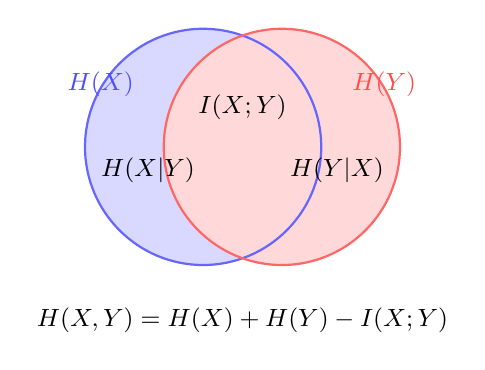
\begin{tikzpicture}[
    mycircle/.style={circle, draw=blue!60, fill=blue!10, minimum size=2.5cm, thick},
    mylabel/.style={font=\small}
]
    % Venn diagram
    \begin{scope}
        \fill[blue!15] (-0.5, 0) circle (1.5cm);
        \fill[red!15] (0.5, 0) circle (1.5cm);
        \draw[blue!60, thick] (-0.5, 0) circle (1.5cm);
        \draw[red!60, thick] (0.5, 0) circle (1.5cm);

        \node[mylabel, blue!70] at (-1.8, 0.8) {$H(X)$};
        \node[mylabel, red!70] at (1.8, 0.8) {$H(Y)$};
        \node[mylabel] at (0, 0.5) {$I(X;Y)$};
        \node[mylabel] at (-1.2, -0.3) {$H(X|Y)$};
        \node[mylabel] at (1.2, -0.3) {$H(Y|X)$};

        \node[mylabel] at (0, -2.2) {$H(X,Y) = H(X) + H(Y) - I(X;Y)$};
    \end{scope}
\end{tikzpicture}
\caption{熵与互信息关系的韦恩图。$H(X,Y)$ 是联合熵，$I(X;Y)$ 是互信息（交集），$H(X\mid Y)$ 和 $H(Y\mid X)$ 是条件熵。}
\label{fig:information-theory}
\end{figure}

\begin{mycode}{Python中的信息论计算}
\begin{lstlisting}[language=Python]
import numpy as np

def entropy(probs):
    """计算离散分布的熵"""
    probs = np.asarray(probs)
    probs = probs[probs > 0]  # 排除零概率避免log(0)
    return -np.sum(probs * np.log2(probs))

def kl_divergence(p, q):
    """KL散度 D_KL(p||q)"""
    p = np.asarray(p); q = np.asarray(q)
    mask = p > 0
    return np.sum(p[mask] * np.log2(p[mask] / q[mask]))

def cross_entropy(p, q):
    """交叉熵 H(p, q)"""
    p = np.asarray(p); q = np.asarray(q)
    mask = p > 0
    return -np.sum(p[mask] * np.log2(q[mask]))

# 示例
p = np.array([0.1, 0.2, 0.7])      # 真实分布
q1 = np.array([0.1, 0.2, 0.7])     # 完美预测
q2 = np.array([0.3, 0.3, 0.4])     # 不准确预测

print(f"H(p) = {entropy(p):.4f}")
print(f"D_KL(p||q1) = {kl_divergence(p, q1):.6f} (完美，应为0)")
print(f"D_KL(p||q2) = {kl_divergence(p, q2):.4f}")
print(f"H(p, q1) = {cross_entropy(p, q1):.4f}")
print(f"H(p, q2) = {cross_entropy(p, q2):.4f}")

# 正态分布的微分熵
sigma = 2.0
diff_entropy = 0.5 * np.log(2 * np.pi * np.e * sigma**2)
print(f"\nN(0,{sigma**2}) 的微分熵: {diff_entropy:.4f}")

# 互信息示例
# P(X,Y) 联合分布
joint = np.array([
    [0.25, 0.10],
    [0.15, 0.50]
])
px = joint.sum(axis=1)
py = joint.sum(axis=0)
mutual_info = 0
for i in range(2):
    for j in range(2):
        if joint[i, j] > 0:
            mutual_info += joint[i, j] * np.log2(
                joint[i, j] / (px[i] * py[j])
            )
print(f"互信息 I(X;Y) = {mutual_info:.4f}")
\end{lstlisting}
\end{mycode}

\section{最大似然估计}

\subsection{似然函数}

给定独立同分布的观测数据 $\mathcal{D}=\{\mathbf{x}^{(1)},\mathbf{x}^{(2)},\ldots,\mathbf{x}^{(m)}\}$，以及参数为 $\boldsymbol{\theta}$ 的模型，似然函数为：

\[
L(\boldsymbol{\theta}) = P(\mathcal{D}\mid\boldsymbol{\theta}) = \prod_{i=1}^{m} p(\mathbf{x}^{(i)}\mid\boldsymbol{\theta})
\]

对数似然函数通常更方便优化：
\[
\ell(\boldsymbol{\theta}) = \log L(\boldsymbol{\theta}) = \sum_{i=1}^{m} \log p(\mathbf{x}^{(i)}\mid\boldsymbol{\theta})
\]

\subsection{最大似然估计}

最大似然估计（Maximum Likelihood Estimation, MLE）选择使观测数据出现概率最大的参数：

\[
\boldsymbol{\theta}_{\mathrm{MLE}} = \arg\max_{\boldsymbol{\theta}} L(\boldsymbol{\theta}) = \arg\max_{\boldsymbol{\theta}} \sum_{i=1}^{m} \log p(\mathbf{x}^{(i)}\mid\boldsymbol{\theta})
\]

MLE 具有优良的渐近性质：当样本量趋于无穷时，MLE 是一致的（收敛到真值）和渐近有效的（达到 Cramér-Rao 下界）。

\subsection{MLE 与损失函数}

许多常用的损失函数可以从 MLE 的角度推导：

\begin{itemize}
    \item \textbf{均方误差（MSE）}：假设目标值 $y$ 服从以模型输出为均值、固定方差的高斯分布，即 $p(y\mid\mathbf{x},\boldsymbol{\theta})=\mathcal{N}(f(\mathbf{x};\boldsymbol{\theta}),\sigma^2)$。其负对数似然正比于 $\sum_{i}(y_i-f(\mathbf{x}^{(i)}))^2$，即 MSE 损失。
    \item \textbf{交叉熵损失}：假设输出服从类别分布（Categorical distribution），$p(y\mid\mathbf{x},\boldsymbol{\theta})=\prod_{k=1}^{K}(\hat{y}_k)^{\mathbf{1}_{y=k}}$。负对数似然为 $-\sum_{i}\log \hat{y}_{y_i}$，即交叉熵损失。
\end{itemize}

因此，最小化 MSE 等价于在高斯噪声假设下的 MLE，最小化交叉熵等价于在类别分布假设下的 MLE。

\begin{mycode}{Python中的MLE示例}
\begin{lstlisting}[language=Python]
import numpy as np
from scipy.optimize import minimize

# 从 N(mu=5, sigma=2) 生成数据
np.random.seed(42)
true_mu, true_sigma = 5.0, 2.0
data = np.random.normal(true_mu, true_sigma, 1000)

# 负对数似然函数
def neg_log_likelihood(params):
    mu, sigma = params[0], params[1]
    if sigma <= 0:
        return np.inf
    n = len(data)
    # -log L = n*log(sqrt(2*pi)*sigma) + sum((x-mu)^2)/(2*sigma^2)
    nll = n * np.log(np.sqrt(2 * np.pi) * sigma)
    nll += np.sum((data - mu) ** 2) / (2 * sigma ** 2)
    return nll

# 优化
result = minimize(neg_log_likelihood, x0=[0, 1],
                  bounds=[(None, None), (1e-6, None)])
mu_hat, sigma_hat = result.x
print(f"真实参数: mu={true_mu}, sigma={true_sigma}")
print(f"MLE估计: mu={mu_hat:.4f}, sigma={sigma_hat:.4f}")

# 验证：样本均值和样本标准差应为MLE
print(f"\n样本均值: {data.mean():.4f}")
print(f"样本标准差 (MLE, 除以n): {data.std(ddof=0):.4f}")
print(f"样本标准差 (无偏, 除以n-1): {data.std(ddof=1):.4f}")
\end{lstlisting}
\end{mycode}

\section{最大后验估计}

MLE 只考虑似然，忽略了参数的先验信息。最大后验估计（Maximum A Posteriori, MAP）结合先验分布和似然：

\[
\boldsymbol{\theta}_{\mathrm{MAP}} = \arg\max_{\boldsymbol{\theta}} P(\boldsymbol{\theta}\mid\mathcal{D})
= \arg\max_{\boldsymbol{\theta}} P(\mathcal{D}\mid\boldsymbol{\theta})P(\boldsymbol{\theta})
\]

取对数：
\[
\boldsymbol{\theta}_{\mathrm{MAP}} = \arg\max_{\boldsymbol{\theta}} \left[\log P(\mathcal{D}\mid\boldsymbol{\theta}) + \log P(\boldsymbol{\theta})\right]
\]

MAP 与正则化的关系：
\begin{itemize}
    \item \textbf{高斯先验} $P(\mathbf{w})\propto\exp(-\frac{\|\mathbf{w}\|^2}{2\sigma^2})$ 对应 $L^2$ 正则化（权重衰减）
    \item \textbf{Laplace 先验} $P(\mathbf{w})\propto\exp(-\frac{\|\mathbf{w}\|_1}{\sigma})$ 对应 $L^1$ 正则化（稀疏化）
\end{itemize}

这为正则化提供了贝叶斯解释：正则化项实际上是参数先验分布的对数。

\section{随机过程初步}

\subsection{马尔可夫链}

马尔可夫链是一类重要的随机过程，满足马尔可夫性质：给定当前状态，未来状态与过去状态条件独立。即：

\[
P(X_{t+1}=x_{t+1}\mid X_t=x_t, X_{t-1}=x_{t-1},\ldots,X_1=x_1) = P(X_{t+1}=x_{t+1}\mid X_t=x_t)
\]

马尔可夫链在深度学习中的应用包括：
\begin{itemize}
    \item MCMC（Markov Chain Monte Carlo）采样方法
    \item 强化学习中的马尔可夫决策过程（MDP）
    \item RNN/Transformer 中的自回归序列建模
\end{itemize}

\section{本章小结}

本章介绍了深度学习所需的概率与统计基础知识：
\begin{itemize}
    \item 随机变量分为离散和连续两类，分别用PMF和PDF描述
    \item 正态分布在深度学习中无处不在，从权重初始化到批归一化
    \item 贝叶斯定理是连接先验、似然和后验的桥梁，为正则化提供了概率解释
    \item 期望、方差和协方差是对随机变量进行定量分析的基本工具
    \item 信息论中的熵、KL散度和交叉熵是理解分类损失函数的关键
    \item MLE和MAP将参数估计与损失函数优化统一在概率框架下
\end{itemize}

扎实的概率统计基础有助于理解深度学习的损失函数设计、生成模型和贝叶斯方法。
